
\begin{comment}%%
\section{Tritium as a Calibration Source}

Due to the self shielding properties of liquid xenon it is practically impossible to perform a low energy electronic recoil (ER) calibration within the fiducial volume of a +100 kg detector using an external source. The fiducial volume of the LUX detector is surrounded by more than than 6 cm of liquid xenon providing excellent shielding from both external backgrounds and calibration sources. For example, a 100 keV gamma has a mean free path of about 2 mm in liquid xenon and would require thirty mean free paths to penetrate into the fiducial volume. A higher energy source such as $\rm ^{137}Cs$ (662 keV) has a longer mean free path of 4 cm however, the probability of a low energy deposit from forward scattering is greatly suppressed. Further, calibrating within the fiducial volume by relying on gammas from an external source to forward scatter brings along systematic uncertainties from high energy deposits near the edge, DAQ rate and having to use  multi scatter event selection instead of a standard set of single scatter WIMP search cuts. An ideal ER calibration source for current and next generation noble gas detectors should consist of single scatter events depositing sub 10 keV energies uniformly distributed in the fiducial region. These requirements are all satisfied by tritium beta decay. Tritium has a Q value of 18.6 keV \cite{Tritium_Q}, a mean beta energy of 5.6 keV \cite{Tritium_Mean} and a mode of 3 keV \cite{Tritium_Eq} making it an ideal low energy internal calibration source, so long as it can removed after calibration. The half-life of tritium is 12.3 years \cite{Tritium_halflife_all} thus it is not practical to wait for the activity to decay away as with other standard internal calibration sources [kr83 ref], the tritium must be removed after the calibration is complete. To mitigate the effect of tritium diffusion into plastics we use tritiated methane instead of bare tritium. For tritiated methane, a tritium atom along with three hydrogen atoms are bound to a carbon molecule. Using tritiated methane lessens the diffusion of tritium into detector internals by an order of magnitude \cite{miyake:1983}. The weak molecular bond, sub on eV, to the methane molecule does not impact the nuclear physics of the tritium beta decay. We have studied the removal of methane by the commonly used SAES heated zirconium getter and found that significant amounts of methane can be removed from xenon at flow rates commonly employed in large scale liquid xenon experiments \cite{Dobi_CH4},\cite{coldtrap}.

\end{comment}%%
%%

\section{Results from the Tritiated Methane Calibration}

\subsection{Tritiated Methane injection into the LUX detector}

In the experimental setup at UMD it was demonstrated that tritiated methane could be injected directly into a liquid xenon vessel containing plastics and removed [link section in this paper]. However, even with conservative estimates of diffusion rates into mock plastic components we could not be certain about the diffusion of methane in the much larger LUX detector. Having the xenon gas sampling system, developed for LUX to track krypton \cite{Kr_ppt_Dobi} \cite{EXO_SAM}, allowed us to conduct situ methane measurements providing a diagnostic of the natural methane diffusion and outgassing without the risk of permanent tritium contamination. Before injecting triturated methane into the detector we first injected $\rm 1/10^{6}$ (g/g) of methane and demonstrated its removal from the LUX xenon to five orders of magnitude, this allowed us to proceed with confidence knowing that the goal of reducing the tritium rate to less than 5\% of background could be met. Methane is chemically identical to tritiated methane and having the ability to sample the gas proved useful for the tritium campaign, the purification time constant for methane removal was measured to be $\rm 5.9 \pm 0.07$ hours with the xenon gas sampling system \ref{fig:Removal_methane}. The removal time constant was $\rm 1/5$ of that expected based on xenon circulation rates alone, potentially enhanced by the solubility of methane between the liquid and gaseous xenon. The enhanced purification time constant allowed for larger injections of tritiated methane into the detector.  (INSERT JON'S PURIFICATION TIME CONSTANT PLOT)


Following the natural methane test the tritiated methane injection was conducted. An absolute activity of 20 mBq of tritiated methane was injected at the purifier's outlet while circulating. A removal time constant of $\rm 6.0 \pm 0.5$ hours was measured in the liquid volume consistent with the natural methane removal measured in the gas by the sampling system, \ref{fig:Removal}. After a day of circulating through the getter the tritium rate had fallen below detectable levels confirming the effective removal of the tritiated methane with the getter. A second, larger injection of 800 mBq was performed a week later yielding a similar removal time constant of $\rm 6.4 \pm 0.1$. The second injection produced 20,000 beta decays in the LUX detector before being completely removed, 7000 of those decays were in the fiducial volume and were used to calibrate the ER band in the WIMP search region of 1-50 Phe (about 1-8 $\rm keV{ee}$). The new tritium calibration source provided an unprecedented low energy electronic recoil calibration for the LUX dark matter search \cite{LUX_PRL}. The injections were performed while circulating and with the getter actively purifying in order maintain detector purity and stability. Prior to LUX detector upgrades in December of 2013 a total of 10 Bq of tritiated methane was injected into the LUX detector and successfully removed providing over 150,000 beta decays within the fiducial volume. 

%The $\rm CH_3T$ (tritiated methane) was injected at the getter output and had passed through a special methane purifier to remove $\rm O_2$, $\rm H_2O$ and other electronegative impurities that could cause a degradation in election lifetime. 

\begin{figure}[h!]\centering
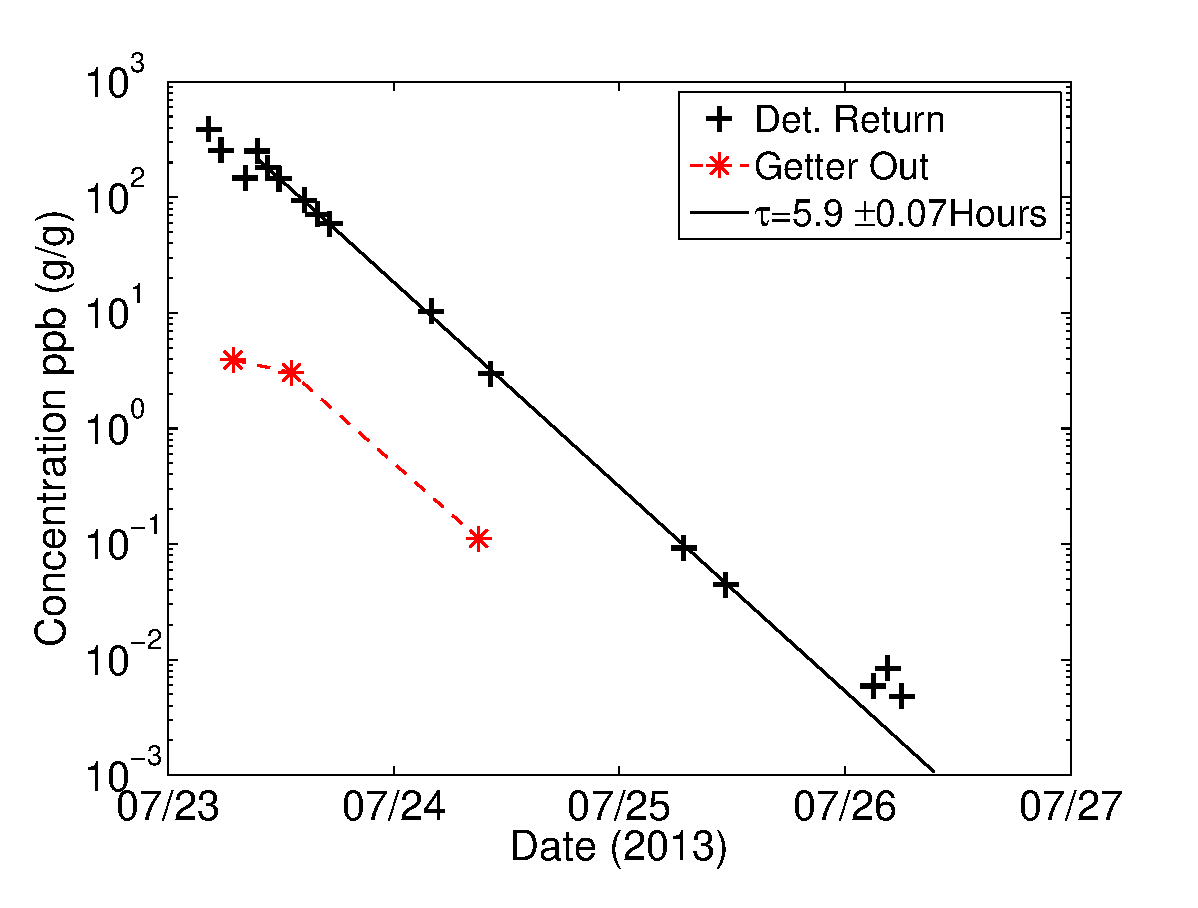
\includegraphics[width=80mm]{CH4_injection_3.eps}
\caption{Removal of natural methane observed by the integrated xenon sampling system prior to the tritiated methane injections. The red points indicate xenon gas measurements at the getter outlet, we find a 97\% one pass removal efficiency at a flow rate of 25 SLPM. $\rm 1\times10^{-3}$ ppb (g/g) is the limit of detection for methane using the LUX gas sampling system.}
\label{fig:Removal_methane}
\end{figure}


\begin{figure}[h!]\centering
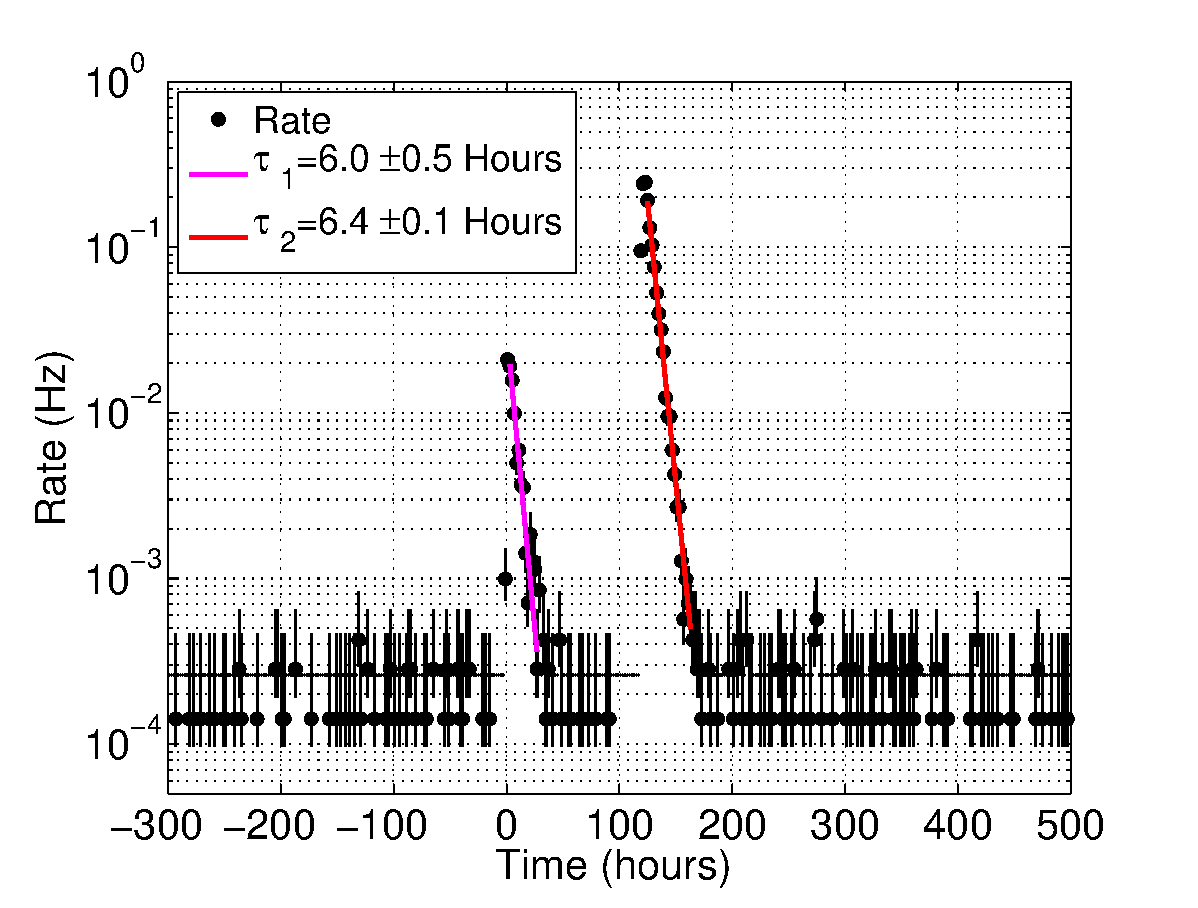
\includegraphics[width=80mm]{CH3T_Rate_fid_150_Run03_Tritium_Rate.eps}
%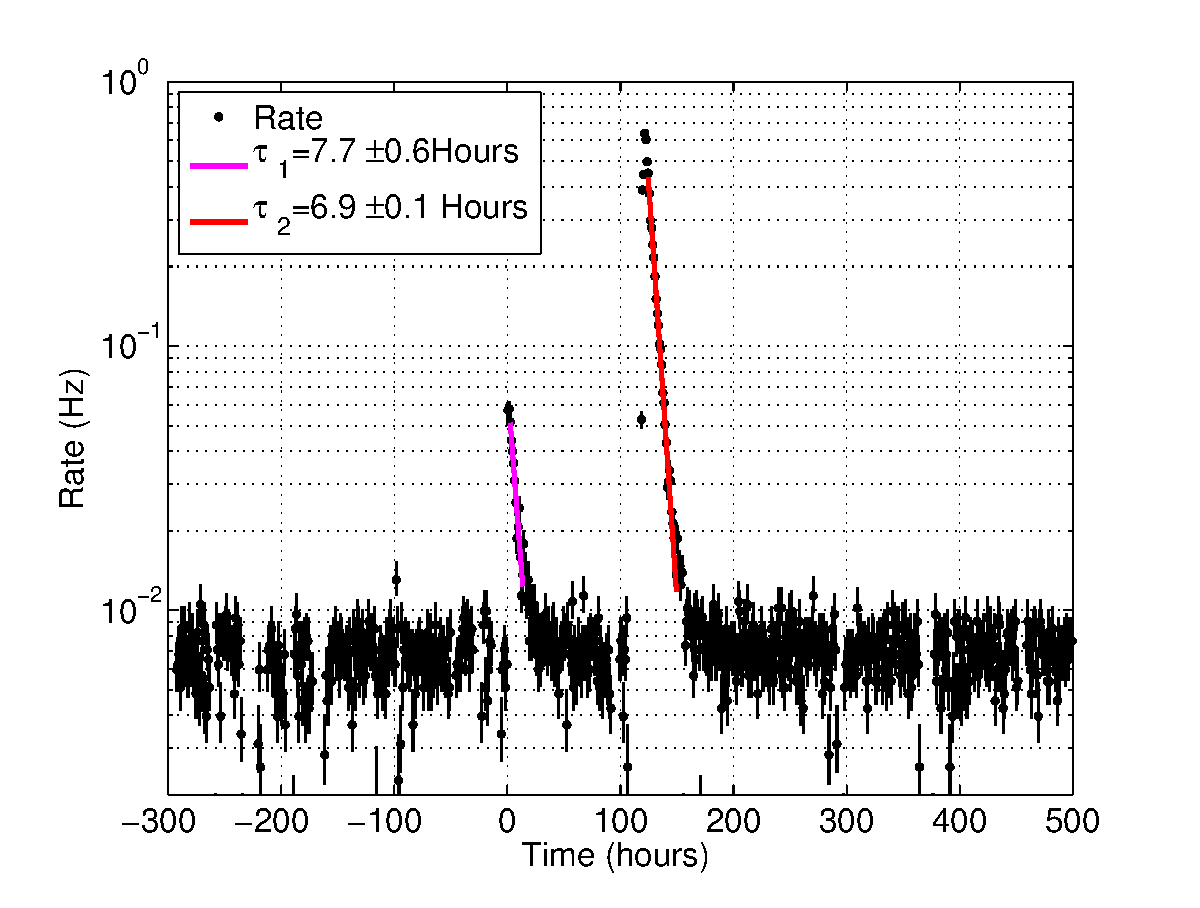
\includegraphics[width=60mm]{CH3T_Rate_Nofid_150_Run03_Tritium_Rate}
\caption{Left: Rate of single scatter events with S1 below 150 Phe in the fiducial volume. 150 Phe in S1 is about 18.6 $\rm keV{ee}$, the endpoint to the tritium beta spectrum. The magenta and red curves are fits to the first and second tritium injection's removal rate. Right: The rate of single scatter events with S1 below 150 for the whole detector volume. Note the removal of tritiated methane is consistent with the natural methane removal rate measured independently.}
\label{fig:Removal}
\end{figure}


\subsection{Mixing of Tritiated Methane in Liquid Xenon}

Tritium events appear uniformly distributed in the liquid volume several minutes after injecting the tritiated methane inline with the xenon gas circulation path. Figure \ref{fig:Density} shows the XY and Z distribution of tritium events thirty minutes after an injection. The events shown cover the region from the gate to the cathode and radially out to the edge of the detector. An additional cut requiring that the event be between $\rm \pm 3 \sigma$ of the ER mean was made to diregard residual alpha events from the walls and cathode, the event rate consisted overwhelmingly of tritium events. The tritiated methane dispersed uniformly throughout the liquid xenon illuminating all regions on the detector and was removed with a time constant consistent with the natural methane. 
 
\begin{figure}[h!]\centering
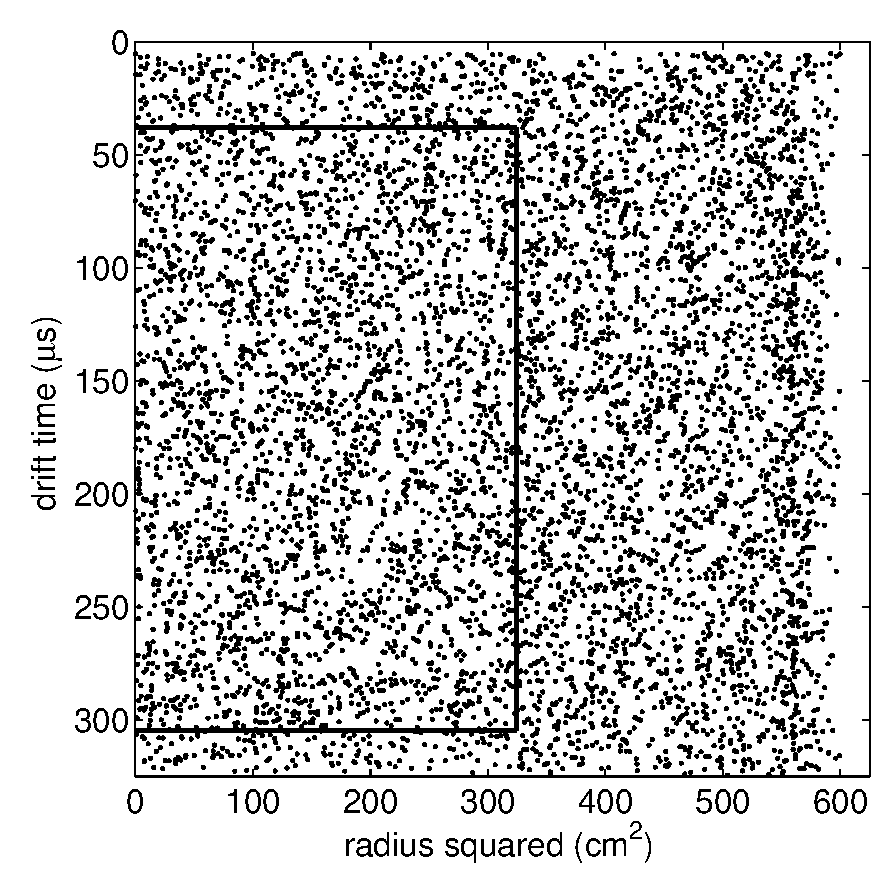
\includegraphics[width=80mm]{CH3T_RZ_scatter_lux10_20130812T1546.eps}
%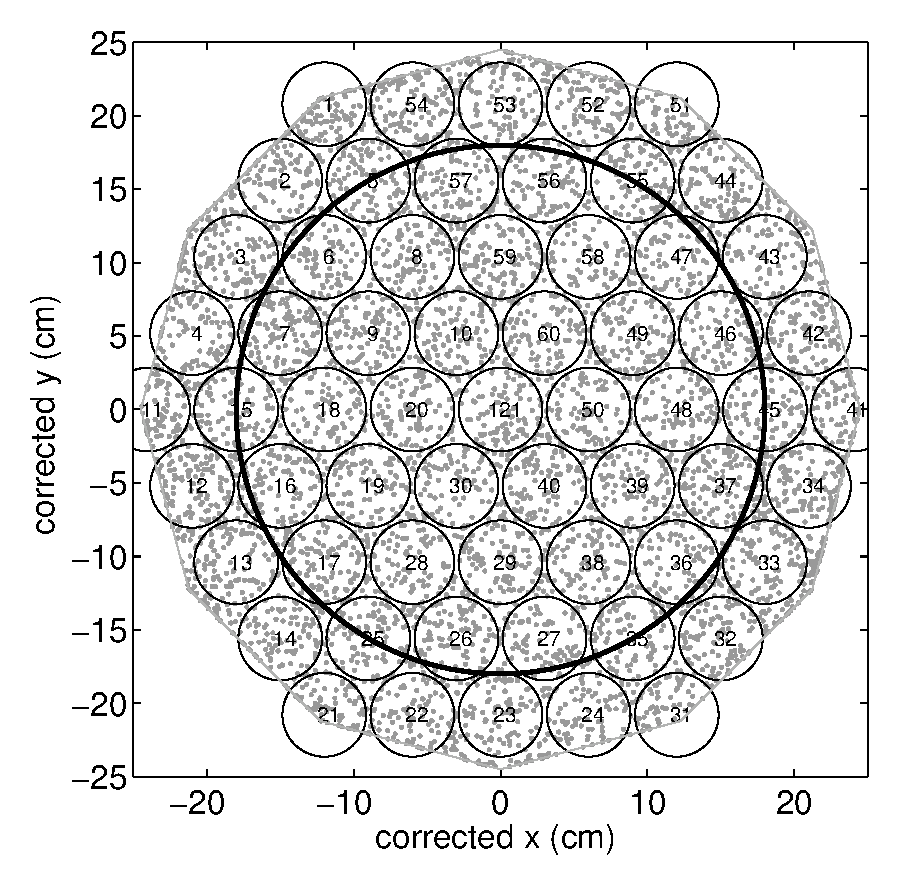
\includegraphics[width=80mm]{CH3T_XY_scatter_PMT_lux10_20130812T1546.eps}
%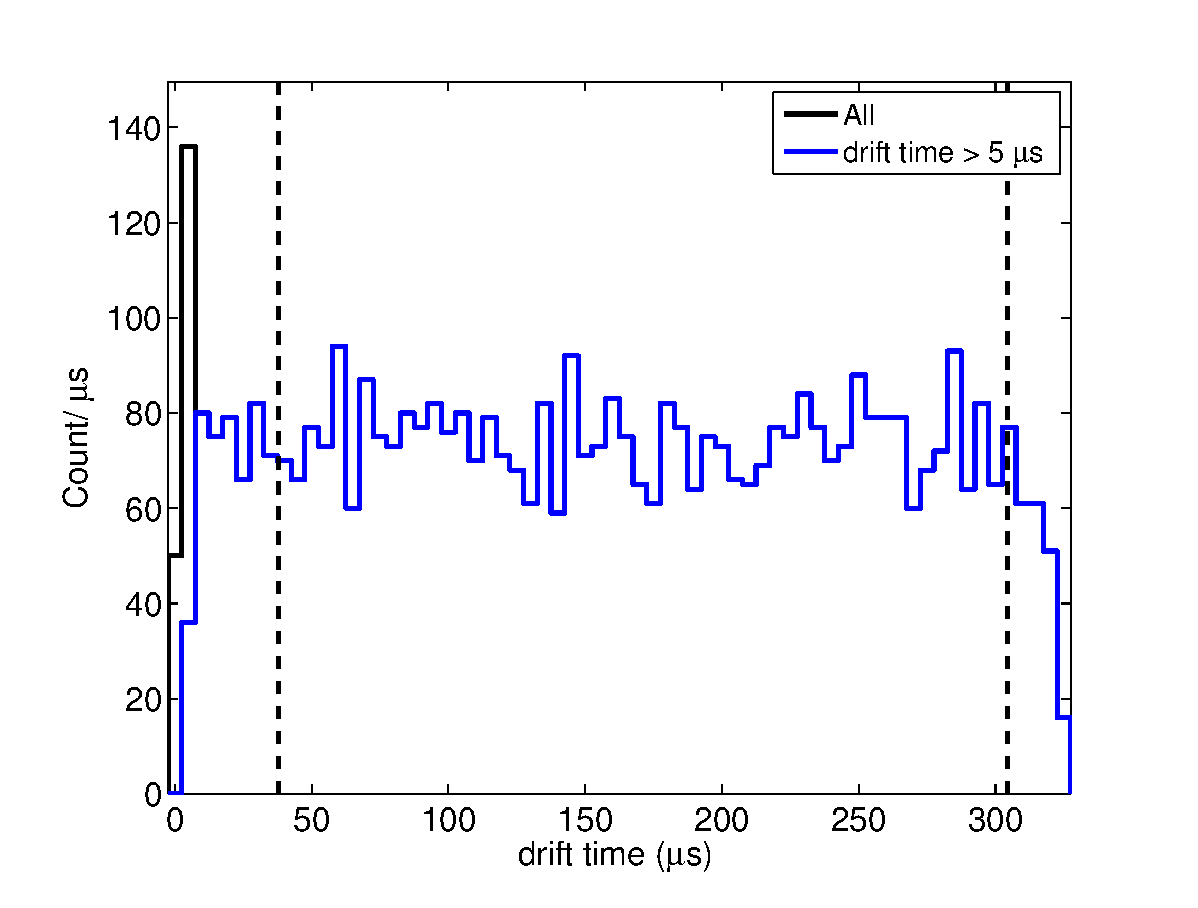
\includegraphics[width=80mm]{CH3T_Z_density_lux10_20130812T1546.eps} %> No Need R^2 vs. Z figure contains Z information
\caption{The distribution of tritium events vs. detector radius squared. The solid black line represents the fiducial volume.
% Right: The distribution of tritium events vs. XY in the region between the gate and the cathode. The solid black line represents the fiducial volume and the black circles represent the locations of PMTs (photo multiplier tubes).
}
\label{fig:Density}
\end{figure}





  \begin{comment}
... Remove this graphic, for smaller tritium injection
\begin{figure}[h!]\centering
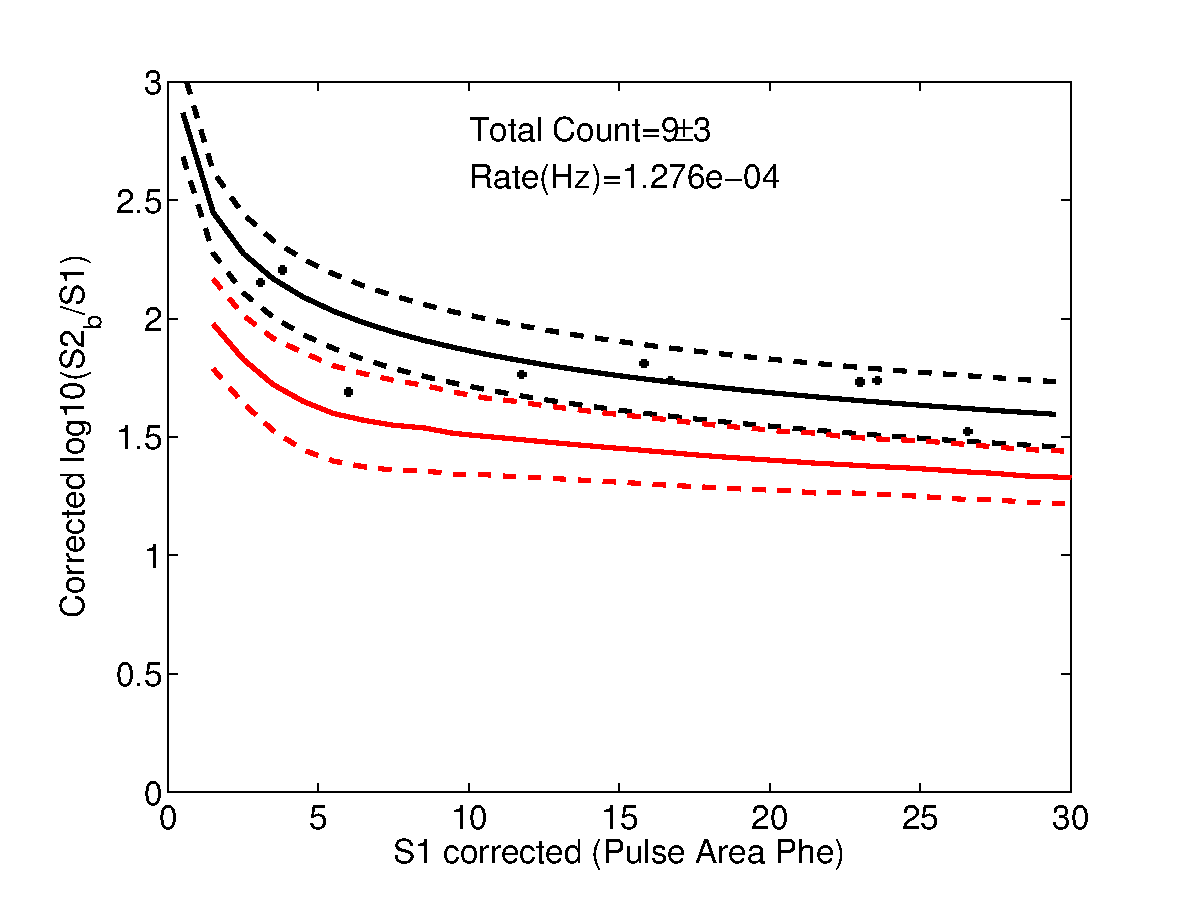
\includegraphics[width=80mm]{CH3T_fid_30_before_100_18_lux10_20130813T1120_cp05328_note.eps}
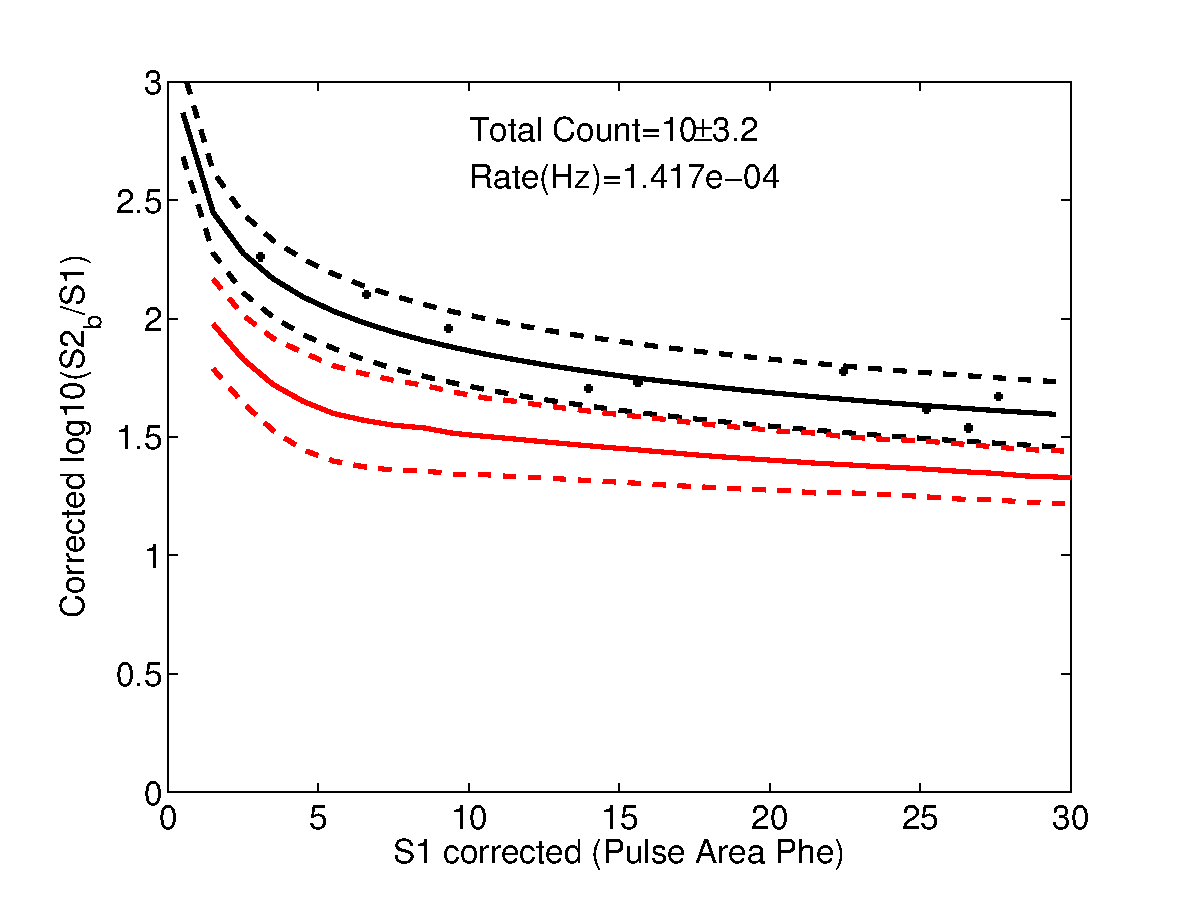
\includegraphics[width=80mm]{CH3T_fid_30_after_100_18_afterlux10_20130813T1120_cp05328_note.eps}
\caption{Left: 100 Hour time window in the WIMP search region before the tritiated methane injection. Right: 100 Hour time window in the WIMP search region after the purification of the tritiated methane. }
\label{fig:Removal_2}
\end{figure}

  \end{comment}

\subsection{Definition of Electronic Recoil Band and Comparison with NEST Model}

Using the tritium source we calibrated the electronic recoil band in the fiducial volume of the LUX detector to unprecedented accuracy. Figure \ref{fig:Band} shows the mean of the ER band along with the 10-90\% confidence bounds ($\pm 1.28\sigma$) obtained from the beta decay of tritium at a drift field of 180 V/cm. The values of the leakage fraction at 50\% NR acceptance per each 1 Phe bins in S1 are shown in \ref{fig:Leak}. The nuclear recoil band, in red, is defined by the NEST model along with AmBe and $\rm^{252}Cf$  calibrations. Methane will not quench xenon scintillation,  even if methane is introduced into the xenon at a relative concentration of a few percent, then the amount of scintillation produced by the mixture is reduced by a factor of two compared to pure xenon \cite{Kirill_Methane}. But for our application we require a methane concentration of only one part in $\rm10^{15}$, and therefore our methane injection will not have any negative effects on scintillation production and transport.

WIMPs primarily interact with the atomic nuclei of xenon atoms in LUX resulting in nuclear recoils whereas the vast majority of residual radioactivity within the detector are gammas which result in electronic recoils. Thus, knowing the separation of the ER from the NR band allows for a measure of the background rejection of a liquid xenon WIMP search experiment. We define the measure of background rejection as leakage fraction, reported here as the fraction of events in the ER band that spill into the lower half of the NR band. Over 115,000 tritium decays were used for the ER band calibration, between 1-50 Phe in S1 (1-8 $\rm keV_{ee}$), and were found using standard WIMP search cuts within the fiducial volume. 
%A figure of merit for ER and NR discrimination is the leakage fraction defined as  the number of tritium events populating the lower half of the NR band are compared to the total number of tritium events in the selected energy range. 
%$\rm (1-erf((Mean\_ER-Mean\_NR)/(sqrt(2)*sigma\_ER)))/2 $.
Figure \ref{fig:Leak} shows the leakage fraction per 1 Phe bins in S1. The mean leakage fraction in the region used for the LUX 2013 PRL results, between 1-30 Phe (1-5 $\rm keV_{ee}$) in the fiducial, was found to be 0.42\% $\rm \pm$ 0.02\%, see Figure \ref{fig:Leak}. In the 40 hour time window in which the data was acquired less than three out of 115,000 events are expected to be non tritium \cite{LUX_BG}. 
%The NR band used is from NEST version 0.98 and is vetted with AmBe, $\rm^{252}Cf$ and DD neutron generator calibrations.


\begin{figure}[h!]\centering
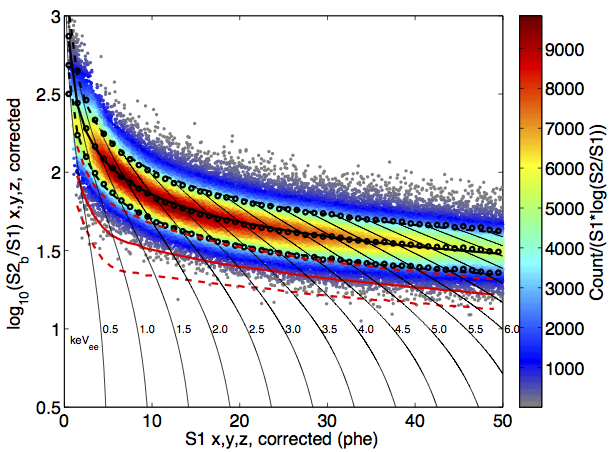
\includegraphics[width=100mm]{CH3T_fid_50_2_Dec_Tritium_Approval_Plots.png}
\caption{Discrimination vs. S1 using over 115,000 tritium beta decays between 1 and 50 Phe in S1 (about $\rm1-8 keV_{ee}$). On average from 1 to 30 Phe the discrimination is 99.58\%, defined by the fraction of events of events below the mean of the nuclear recoil band. The red band represents the NEST nuclear recoil band (version 0.98) vetted with an AmBe, $\rm^{252}Cf$ and DD neutron generator calibration.}
\label{fig:Band}
\end{figure}

\begin{figure}[h!]\centering
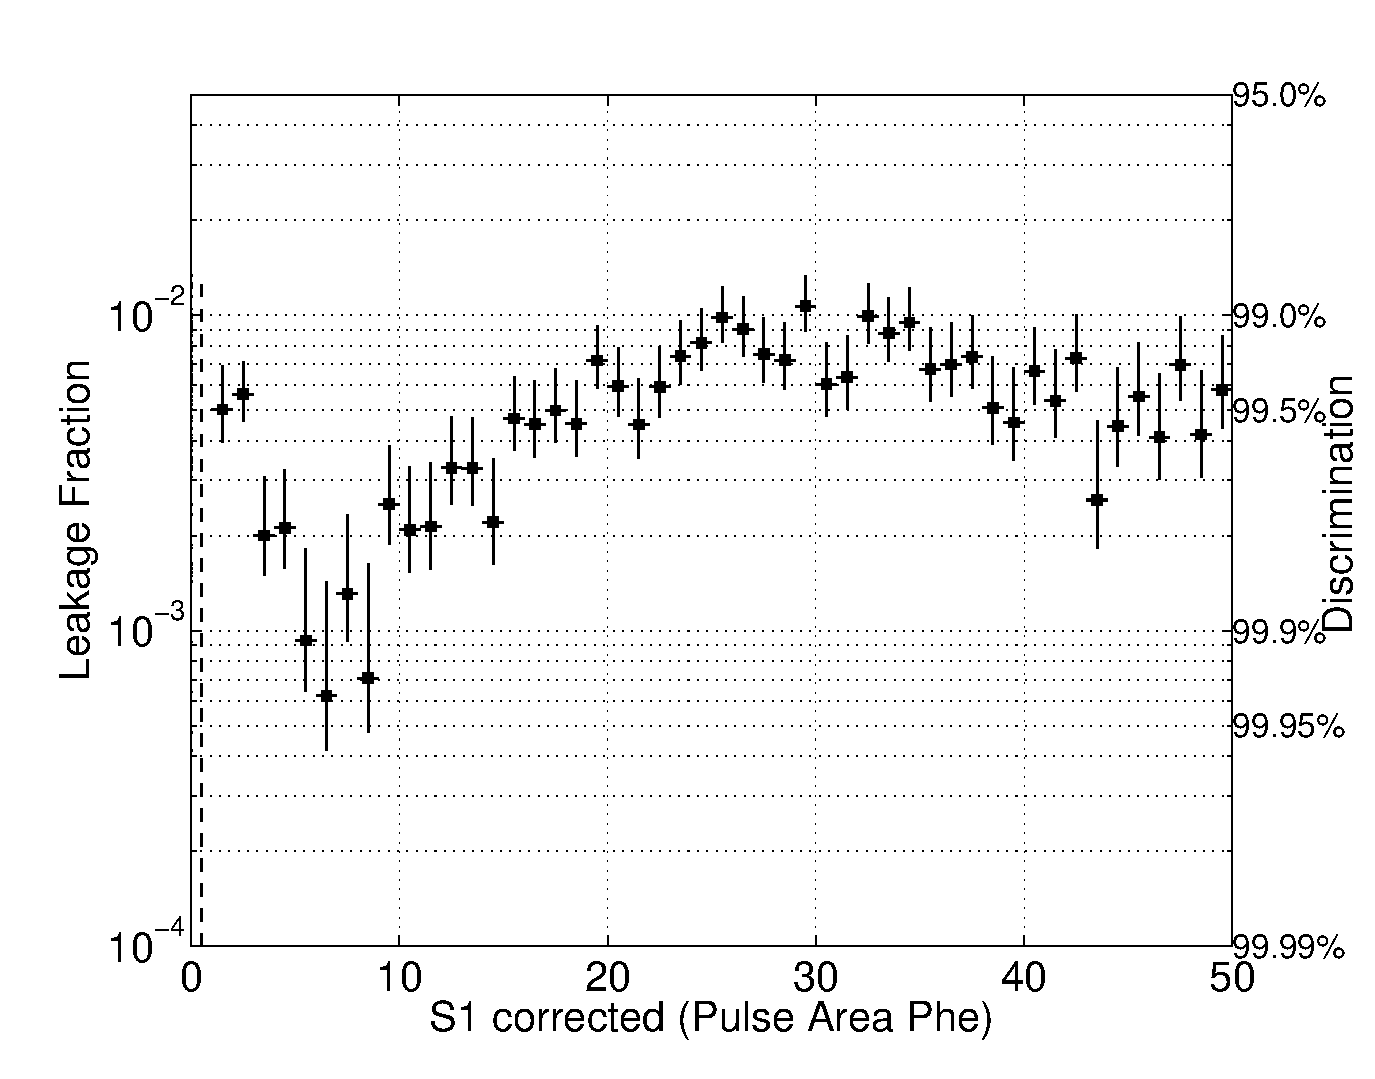
\includegraphics[width=100mm]{CH3T_Leakage_fid_50_Dec_Tritium_Approval_Plots_2.eps}
\caption{Discrimination vs. S1 using over 115,000 tritium beta decays between 1 and 50 Phe in S1 (about $\rm1-8 keV_{ee}$). On average from 1 to 30 Phe the discrimination is 99.58\%, defined by the fraction of events of events below the mean of the nuclear recoil band. The red band represents the NEST nuclear recoil band (version 4c) vetted with an AmBe, $\rm^{252}Cf$ and DD neutron generator calibration.}
\label{fig:Leak}
\end{figure}


%Figure \ref{fig:NEST_v_Data} shows the comparison between simulation(NEST) and the data for the ER band. The agreement between simulation and data is good down to 7 Phe in S1. This is expected since at sub 2 $\rm keV{ee}$ (7 Phe in S1) data is limited and the NEST model has yet to be vetted at such low energies[Matthew/ Erik Dahl Thesis]. The newly acquired ER data below 2 $\rm keV{ee}$ from tritium will be used improve upon the NEST model at the extration field of 180 V/cm [ref?].

\begin{comment}

\begin{figure}[h!]\centering
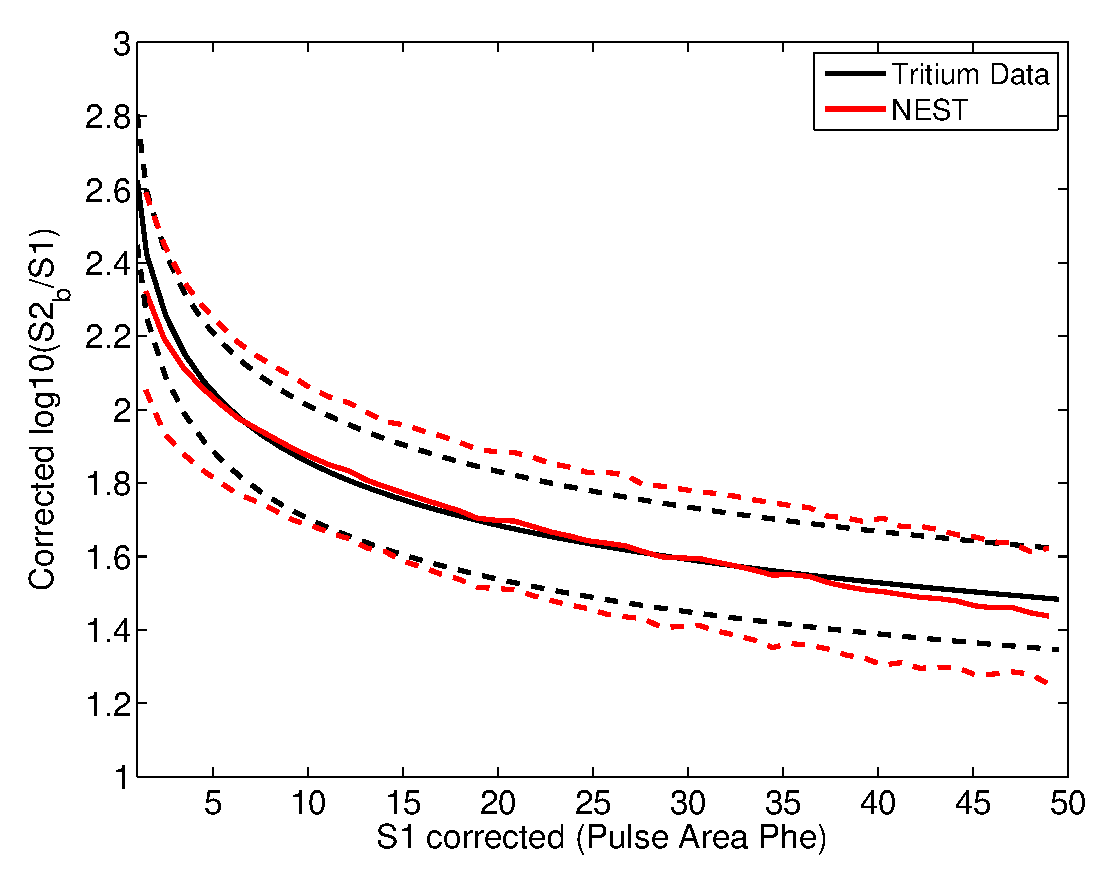
\includegraphics[width=80mm]{CH3T_DATA_NEST_fid_30_LUX_SIM_Tritium.eps}
\caption{ER band measured using tritium data in black with 90\% confidence bounds ( $\rm \pm 1.3 \sigma$) compared with the NEST prediction in red.}
\label{fig:NEST_v_Data}
\end{figure}
\end{comment}

%%%%%%%%%%%%%%%%%%%%%%%%%%%%%%%%%%%%%%%%%%%%%%%%%
\begin{comment}

\subsection{Threshold Determination}

The tritiated methane calibration source can also be used to determine detector efficiency for both S1 (primary scintillation) and S2 (secondary scintillation) down to sub 1 keV electronic recoils.The ultimate limitation of single scatter event is typically the S1 since the signal size of the S1 is one to three orders of magnitude less than the S2. We measured the threshold by comparing the NEST model of a tritium beta spectrum to the data, we find good agreement to the threshold determined from LED calibration, figure \ref{fig:S1S2_Thresh}(need to add to plot). The threshold for the S2 (bottom PMT array) shown is entirely due to the S1 threshold. We use only the bottom PMT array for the S2 signal because the secondary scintillation light is more uniformly distributed along the bottom PMTs than the top PMTs. Figure \ref{fig:E_spec} shows the tritium beta spectrum measured in the LUX detector along with the NEST prediction, note at the 180 V/cm drift field NEST has been vetted form 2 to 10 $\rm keV{ee}$.

\begin{figure}[h!]\centering
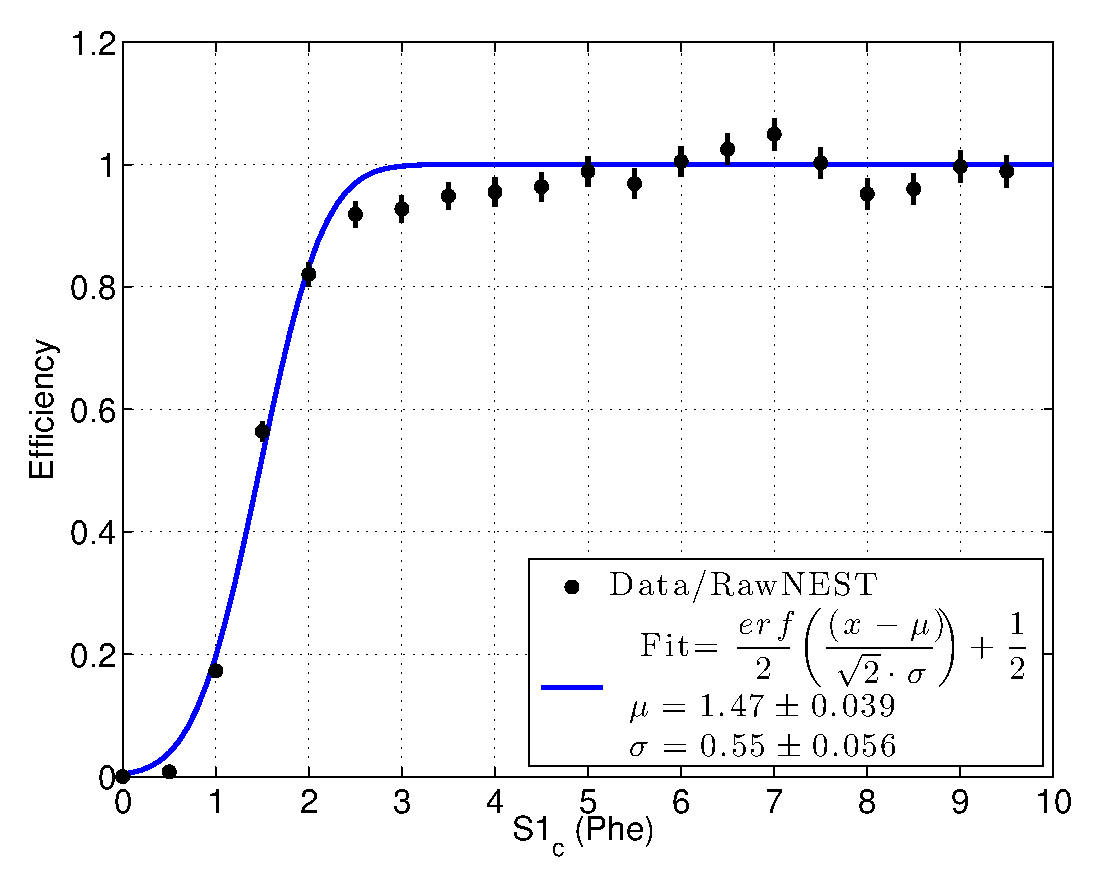
\includegraphics[width=80mm]{CH3T_eff_S1_100_T_paper_corr_threshold.eps}
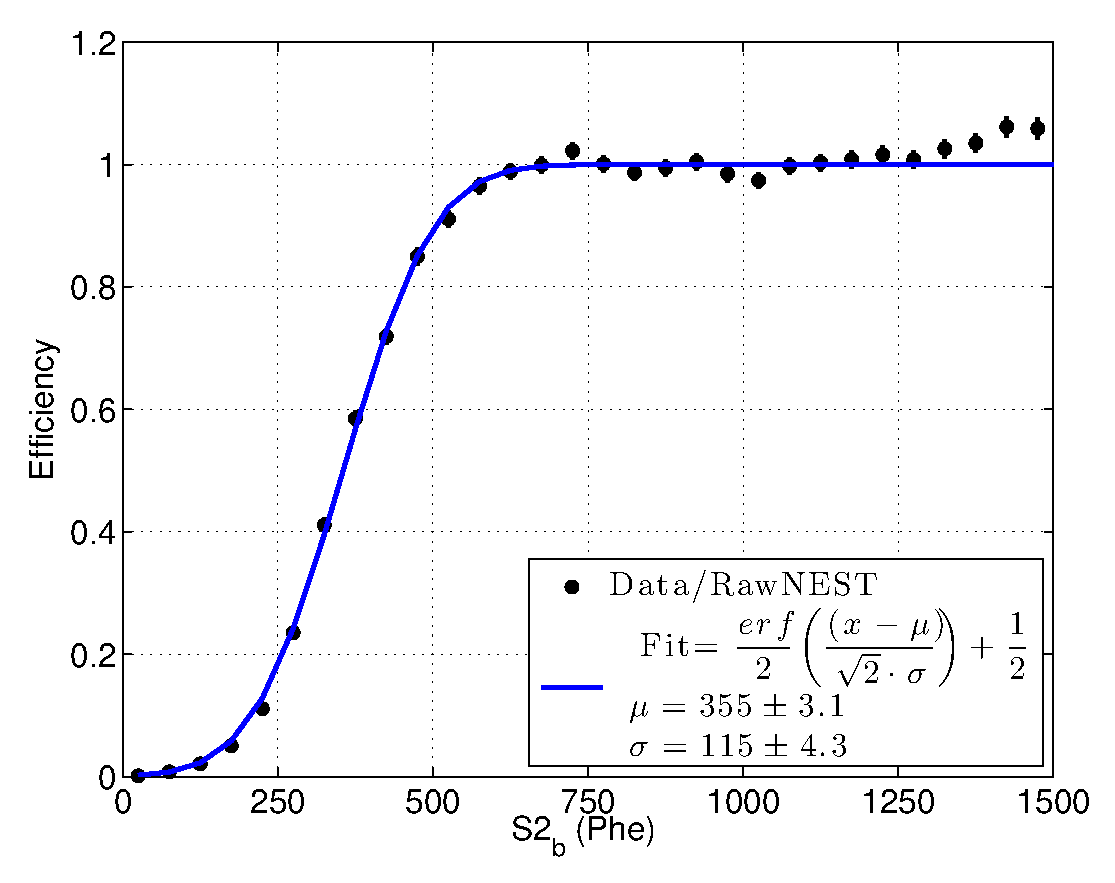
\includegraphics[width=80mm]{CH3T_eff_S2_100_T_paper_corr_threshold.eps}
\caption{S1 Threshold determined from Tritium. S2 Threshold determined from Tritium.}
\label{fig:S1S2_Thresh}
\end{figure}



\begin{figure}[h!]\centering
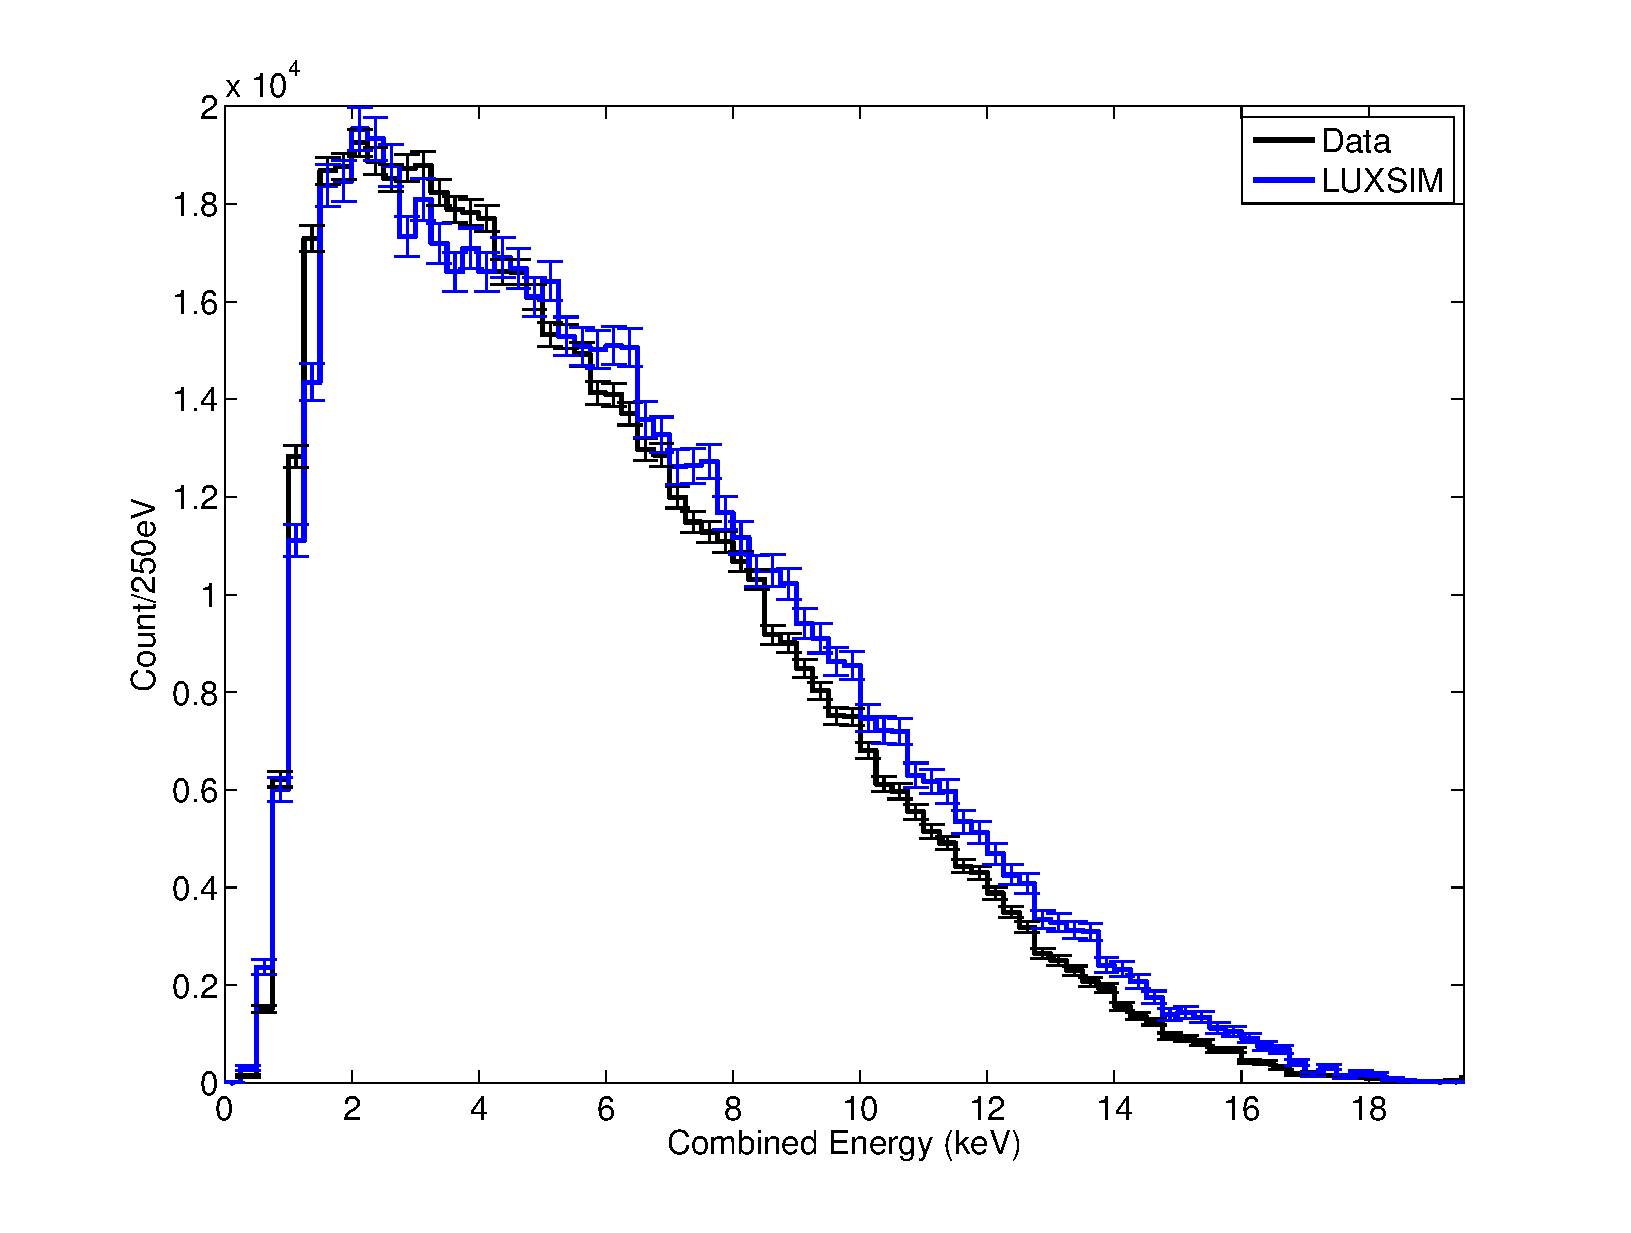
\includegraphics[width=100mm]{CH3T_E_spec_18_Tritium_Dec_2013_180.eps}
\caption{Combined energy spectrum of the tritium data and LUX SIM.}
\label{fig:E_spec}
\end{figure}
 


 
 \subsection{Absolute Rate}
The absolute efficiency for detecting tritium events can be determined by comparing the number of observed events to the number expected. The initial activity injected was calculated to be $0.84 \pm 0.22 $ Bq, with the largest uncertainty coming from the ratio of $\rm CH_3T/CH_4$ from the tritiated methane source bottle. The purification time constant was measured to be 6.6 hours. From the initial rate and the purification constant we expect to count a total of $20,200 \pm 4,000 $ events in the LUX detector before applying the S1 threshold. With the S1 threshold we expect  $16,000 \pm 3,100 $ `golden' events. The actual count observed in the liquid xenon volume was 20,000 events, which is in good agreement with the expected value taking into account the uncertainty in the initial activity and the purification model. After making fiducial cut $7,700 \pm  1,500$ events were expected and a total of $9,500 \pm 100$ were observed.
%,  roughly $16,000 \pm  3,100 * (290/324)*(18^2/24.5^2)$. 



\section{Scintillation Yield and Ionization Yield from Tritium Beta Decay}


\subsection{Cuts used in this analysis}
\begin{itemize}
\item Standard LUX Pulse finder classifier used in the WIMP search.
\item $\rm S2_b > 100 [Phe] $
\item PDE (g1) = 0.138 $\rm \pm 0.005$, measured with Tritium
\item Extraction = 0.664 $\rm \pm 0.04$ measured with Tritium.
\item single e- = 9.95 $\rm \pm 0.1$ [Phe/e-]
\item Using NEST 4c bands.
\end{itemize}




Scintillation and ionization yield are measured using the tritiated methane calibration source from the S1, S2 and reconstructed energy of each beta decay. The energy of each decay is determined using a prescription described in [Erik Dahl], see equations \ref{eq:Gain} and \ref{eq:E_comb}. 
\begin{equation}
\begin{split}
\rm  n_\gamma = \frac{S1}{g1}\\
\rm n_{e^{-}} = \frac{S2}{g2}
\label{eq:Gain}
\end{split}
\end{equation}

\begin{equation}
\begin{split}
\rm E= \frac{1}{W}(n_\gamma + n_{e^-})\\
\rm E= \frac{1}{W}(\frac{S1}{g1} + \frac{S2}{g2})
\label{eq:E_comb}
\end{split}
\end{equation}

The values of the work function W and gains g1, g2 have been measured using other calibration sources and are energy independent [ref]. Using equations \ref{eq:Gain} and \ref{eq:E_comb} we calculate the number of photons and electrons along with the energy of each tritium beta decay event to determine the yields. Scintillation and ionization yield are defined as [Photons/keV] and [Electrons/keV] respectively and the tritiated methane calibration source provides betas ranging from $\rm>1$ to 18 keV, with an exponential decline in event rate above 5 keV. For the results shown in figure \ref{fig:L_Q_Yield_180} over 150,000 beta decays in the fiducial volume were used to measure scintillation and ionization yield at 180 [V/cm]. A correction was applied for the beta spectral shape and the finite resolution of S1, S2 when measuring ionization and scintillation yield, the correction was found to be less than 10\% and is described in [my thesis]. Figure \ref{fig:L_Q_Yield_180} also shows the comparison of the results with the NEST model which has been vetted between 2 and 10 $\rm keV{ee}$. Also show are the measurements of light yield from a $\rm^{83m}Kr$ source, the 32.1 keV decay from $\rm^{83m}Kr$ is typically used as a standard calibration. (The second 9.4 keV decay from $\rm^{83m}Kr$  shown in the figure is for decays that occur more than 1000 ns after the initial 32.1 keV decay).

We find good agreement with the NEST model in the regions that have been vetted (2-10 $\rm keV{ee}$), see figure \ref{fig:L_Q_Yield_180}. Below 2 $\rm keV{ee}$ the light yield is lower than predicted by NEST and the charge yield is higher. The discrepancy between the data and the NEST model above 10 $\rm keV{ee}$ is due to limited data available for the model and also due to the track lengths of betas and gammas beginning to deviate above this energy. Note, under 10 $\rm keV{ee}$ track lengths of betas gammas are nearly identical. 

Figure \ref{fig:L_Q_Yield_Baudis} includes our light and charge yield measurements at 100 and 180 V/cm along with the recent Compton scattering measurement down to 1.5 $\rm keV{ee}$ from \cite{Baudis} at 450 V/cm. The error bars show in the figure include uncertainties from W, g1, g2 and the spectral shape correction. Unlike the measurement made using Compton scattering we can reconstruct energy using both the light and charge channels for each decay allowing for a powerful calibration down to 1 $\rm keV{ee}$ (corresponding to 80\% threshold at 2 Phe in S1).  We find a lower light yield than the centroids of the measurements in [ref Budias], however the the measurement is within reported errors. At our lower fields a higher light yield is expected than that measured at 450 V/cm due to less free charge separation.  The light yield of the 32.1 keV gamma from $\rm^{83m}Kr$ is shown on the figure as a measure of systematic uncertainty between the experiments. For the case of the standardized $\rm^{83m}Kr$ calibration source we find the expected behavior between the two experiments, a higher extraction field leads to lower light yield.

%\begin{figure}[h!]\centering
%\includegraphics[width=120mm]{LY_c_180_Tritium_Dec_2013_Charge_Yield_180_corr.png}
%\includegraphics[width=120mm]{CH3T_fid_E_S2_c_Tritium_Dec_2013_Charge_Yield_180_corr.png}
%\caption{Top: Scintillation yield vs. combined energy using tritium beta decay. Bottom: Ionization yield vs. combined energy using tritium beta decay. At a drift field of 180 [V/cm], in the fiducial volume, and containing over 150,000 beta decays. The endpoint of the tritium beta spectrum is 18.6 [keV]}
%\label{fig:L_Q_Yield}
%\end{figure}


 \begin{figure}[h!]\centering
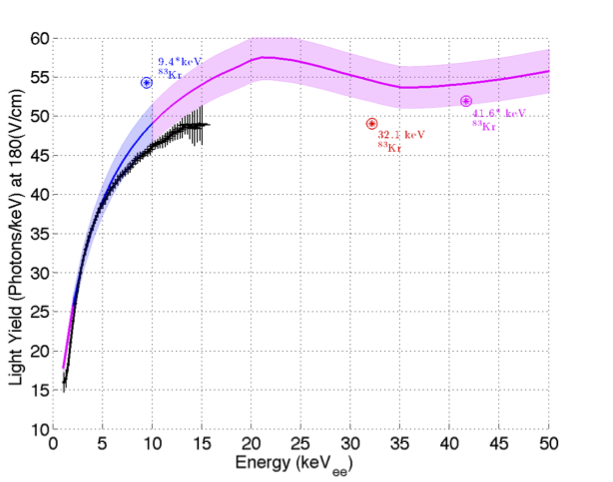
\includegraphics[width=80mm]{LY_180_band_Tritium_Dec_2013_Charge_Yield_180_corr.png}
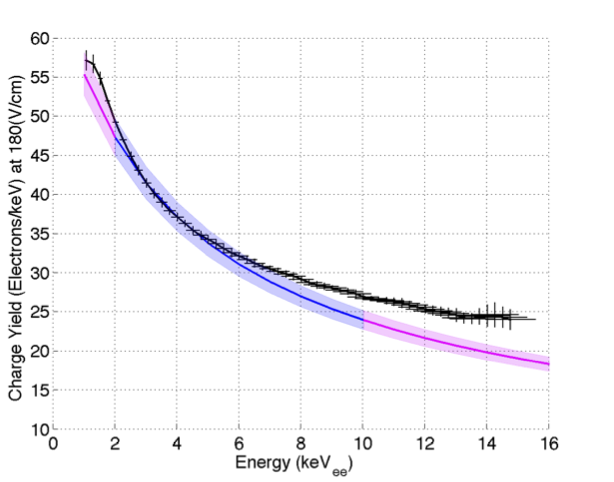
\includegraphics[width=80mm]{QY_180_Tritium_Dec_2013_Charge_Yield_180_corr.png}
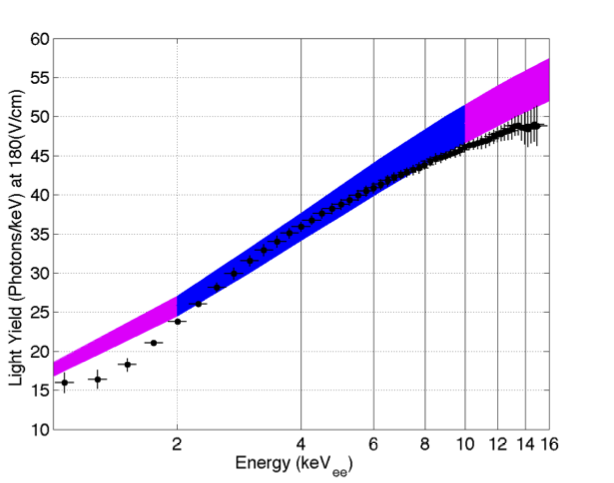
\includegraphics[width=83mm]{LY_180_band_log_Tritium_Dec_2013_Charge_Yield_180_corr.png}
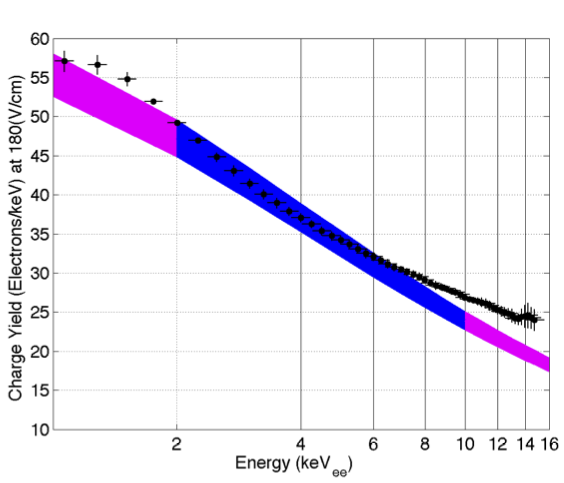
\includegraphics[width=76mm]{QY_180_log_Tritium_Dec_2013_Charge_Yield_180_corr.png}
\caption{180 [V/cm], corrected for spectral shape. Top Left: Mean scintillation yield vs. combined energy using tritium beta decay (black line). $\rm^{83}Kr$ lines are plotted for reference but only the 32.1 [keV] line (red star) is kosher since the 9.4 [keV] line is dependent on timing separation, the 9.4 [keV] line is plotted (blue star) for separations greater than 1000 [ns]. Top Right: Mean ionization yield vs. combined energy (black line). Bottom Left: Scintillation yield vs. combined energy on a log scale. Bottom Right: Ionization yield vs. combined energy on a log scale. The shaded blue regions represent the NEST mean with $\pm 5\%$ that has been vetted by data [Erik Dahl Thesis]. The shaded magenta regions represent the NEST extrapolations from data. The measurement is made at a field of 180 [V/cm] and contains over 150,000 beta decays. The endpoint of the tritium beta spectrum is 18.6 [keV]}
\label{fig:L_Q_Yield_180}
\end{figure}




 \begin{figure}[h!]\centering
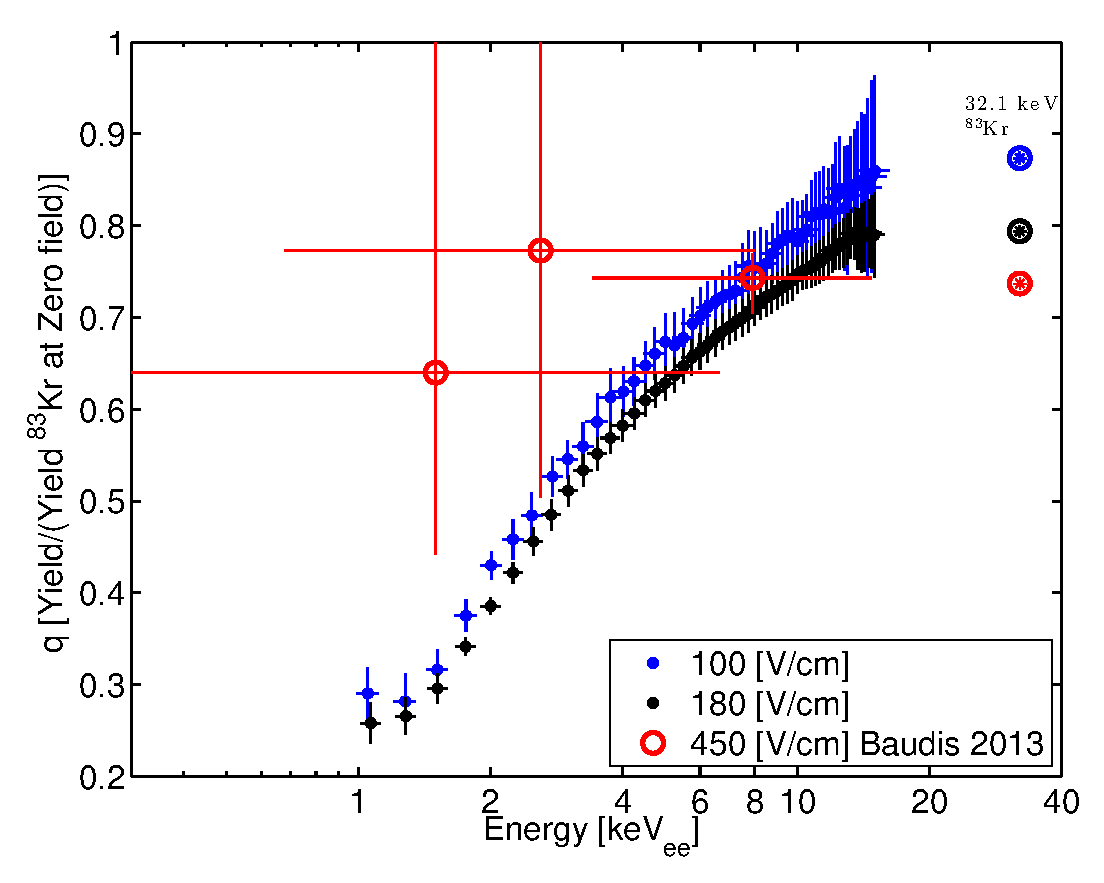
\includegraphics[width=100mm]{q_all_log_Tritium_Dec_2013_Charge_Yield_180_corr.eps}
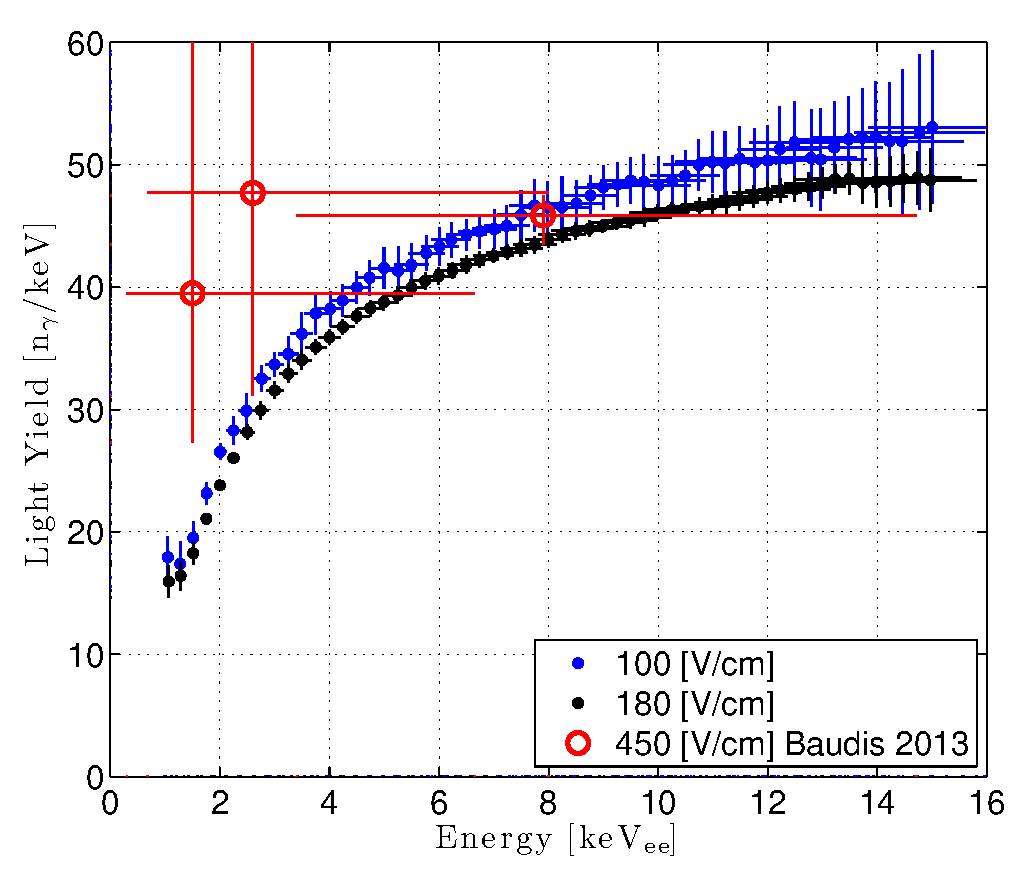
\includegraphics[width=82mm]{LY_all_Tritium_Dec_2013_Charge_Yield_180_corr.eps}
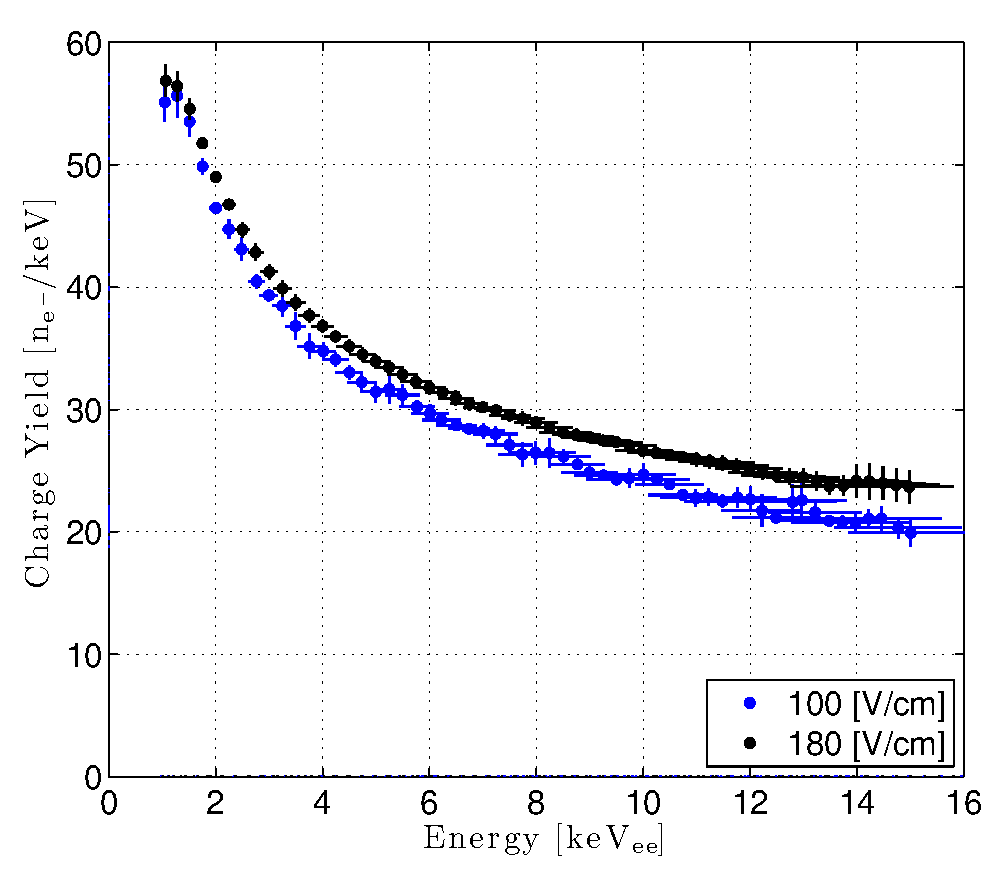
\includegraphics[width=80mm]{Charge_Y_all_Tritium_Dec_2013_Charge_Yield_180_corr.eps}
\caption{Top: Scintillation yield relative to the yield of the 32.1 gamma of [keV] $\rm^{83}Kr $  vs. Energy. Shaded blue curve is tritium at 100 [V/cm], shaded black curve is tritium at 180 [V/cm], red points represent a recent Compton scattering measurement at 450 [V/cm]. Also shown are the corresponding quenching of the 32.1 [keV]  gamma of $\rm^{83}Kr$ (star inside circle). Bottom: scintillation yield [Photons/keV] vs. Energy. Shaded blue curve is tritium at 100 [V/cm], shaded black curve is tritium at 180 [V/cm], red circles represent a recent Compton scattering measurement at 450 [V/cm].}
\label{fig:L_Q_Yield_Baudis}
\end{figure}



\end{comment}
%%%%%%%%%%%%%%%%%%%%%%%%%%%%%%%%%%%%%%%%%%%%%%%%%%%%%%%%%%

\section{All the things we can do with Tritium}

\begin{itemize}
\item Define the ER band.
\item Binned leakage fraction, and potentially optimize for spacial dependent leakage fraction in XYZ plane.
\item S1, S2 threshold. (Energy is a bit convoluted let's not go there). Requires NEST
\item Combined energy calibration to about 0.5 keVee. Requires NEST
\item Light Yield, Charge Yield. Requires some trivial smearing model, 10\% effect.
\item Fano-like factor vs. energy. Requires some trivial smearing model, sub 2\% effect.
\item Fiducial mass calculation, optimized for low energy S2s making it more WIMP like.
\item g1 and g2 calculation by competing tritium spectrum with NEST, or multiple E fields
\item ER band Gaussianity.
\item ... anything else?
\end{itemize}



